\documentclass[11pt,psfig]{article}
\usepackage{epsfig}
\usepackage{times}
\usepackage{amssymb}
\usepackage{float}

\newcount\refno\refno=1
\def\ref{\the\refno \global\advance\refno by 1}
\def\ux{\underline{x}}
\def\ut{\underline{\theta}}
\def\umu{\underline{\mu}}
\def\be{p_e^*}
\newcount\eqnumber\eqnumber=1
\def\eq{\the \eqnumber \global\advance\eqnumber by 1}
\def\eqs{\eq}
\def\eqn{\eqno(\eq)}

 \pagestyle{empty}
\def\baselinestretch{1.1}
\topmargin1in \headsep0.3in
\topmargin0in \oddsidemargin0in \textwidth6.5in \textheight8.5in
\begin{document}
\setlength{\parskip}{1.2ex plus0.3ex minus 0.3ex}


\thispagestyle{empty} \pagestyle{myheadings} \markright{Homework
5: CS 274A, Probabilistic Learning: Winter 2014}



\title{CS 274A Homework 5}
\author{Zachary DeStefano, 15247592}
\date{Due Date: Wednesday March 5th}

\maketitle

 \newpage

\section*{Plots for Dataset1}

\begin{figure}[H]
\centering
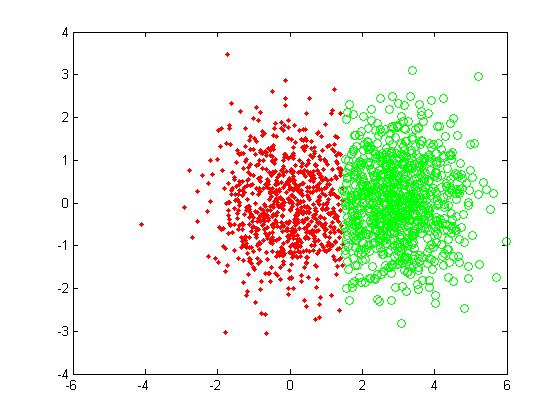
\includegraphics[height=3.25in]{dataset1_kMeansPlot.jpg}
\caption{The k-Means plot for dataset1, K=2}
\end{figure}

\begin{figure}[H]
\centering
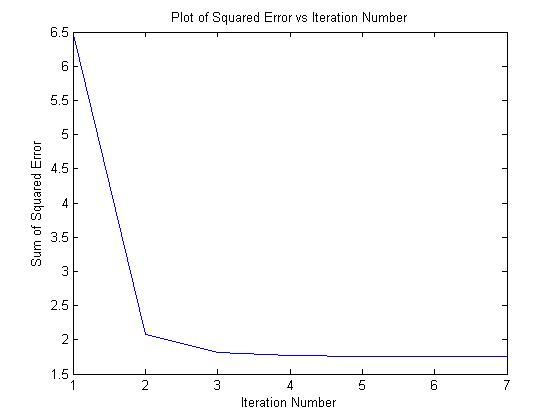
\includegraphics[height=3.25in]{dataset1_kMeans_squaredErrorPlot.jpg}
\caption{The Sum of Squared Error plot for dataset1, K=2}
\end{figure}

\begin{figure}[H]
\centering
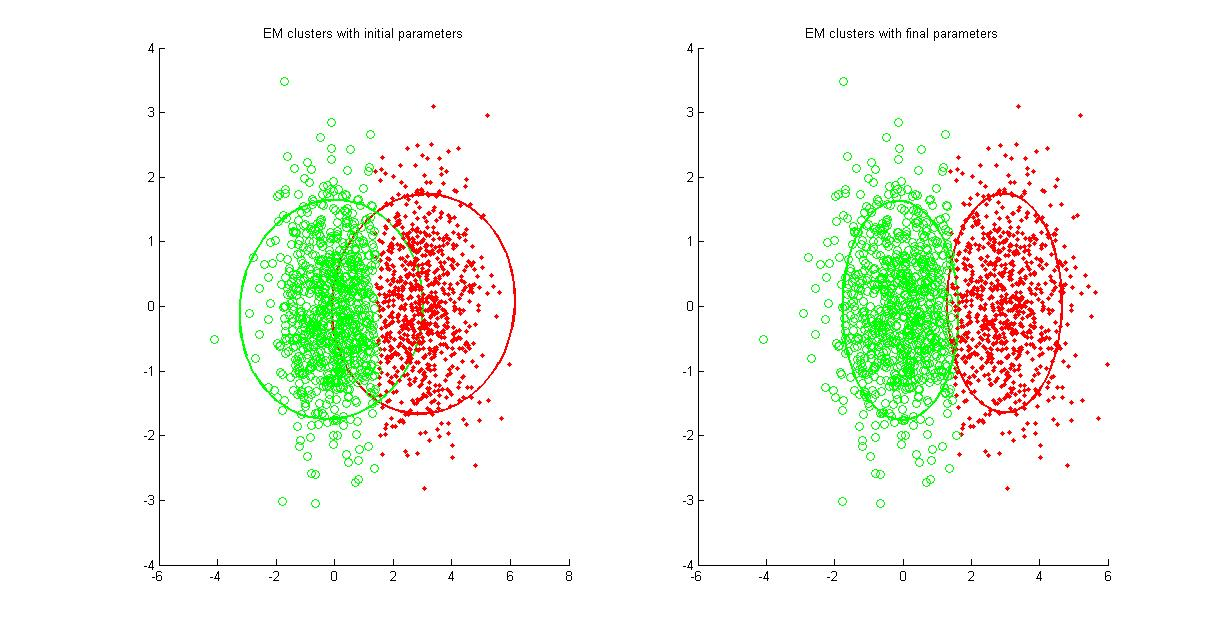
\includegraphics[height=3.25in]{dataset1_EMclusterPlots.jpg}
\caption{The EM cluster plots for dataset1, K=2, using initialization method 3}
\end{figure}

\begin{figure}[H]
\centering
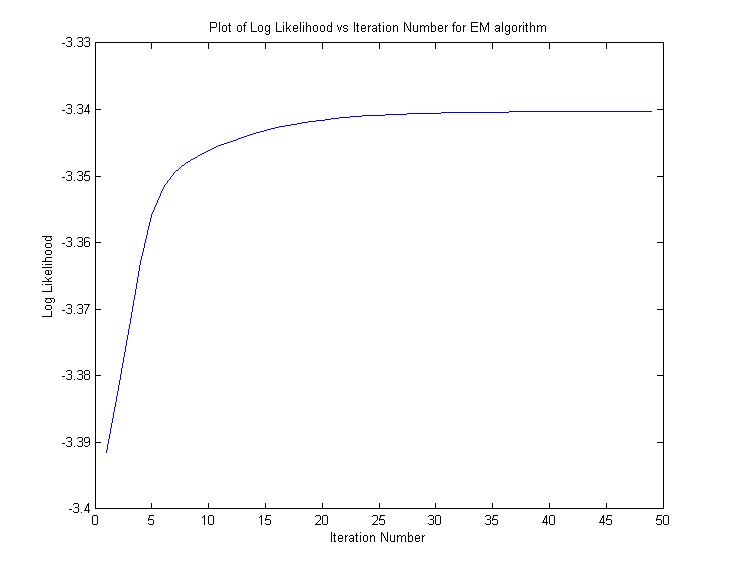
\includegraphics[height=3.25in]{dataset1_EMlogLikelihoodPlot.jpg}
\caption{The likelihood plot for dataset1, K=2, using initialization method 3}
\end{figure}

\section*{Plots for Dataset2}

\begin{figure}[H]
\centering
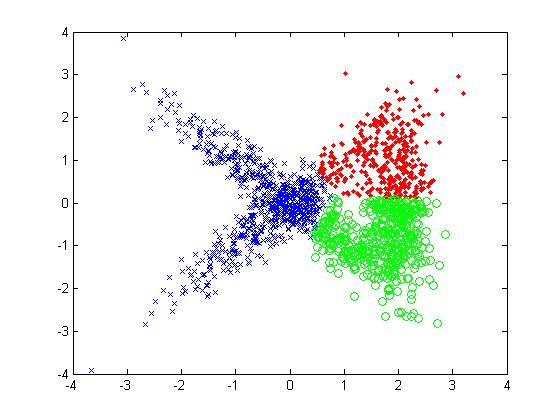
\includegraphics[height=3.25in]{dataset2_kMeansPlot.jpg}
\caption{The k-Means plot for dataset2, K=3}
\end{figure}

\begin{figure}[H]
\centering
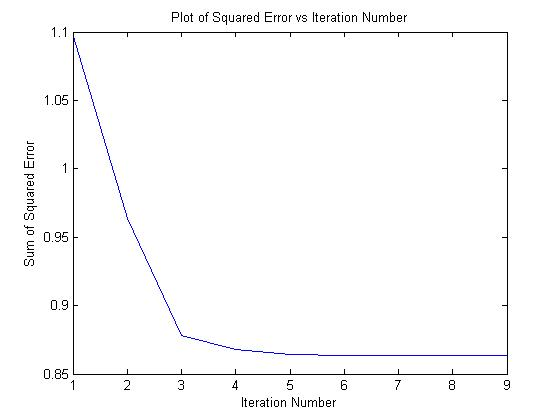
\includegraphics[height=3.25in]{dataset2_kMeans_squaredErrorPlot.jpg}
\caption{The Sum of Squared Error plot for dataset2, K=3}
\end{figure}

\begin{figure}[H]
\centering
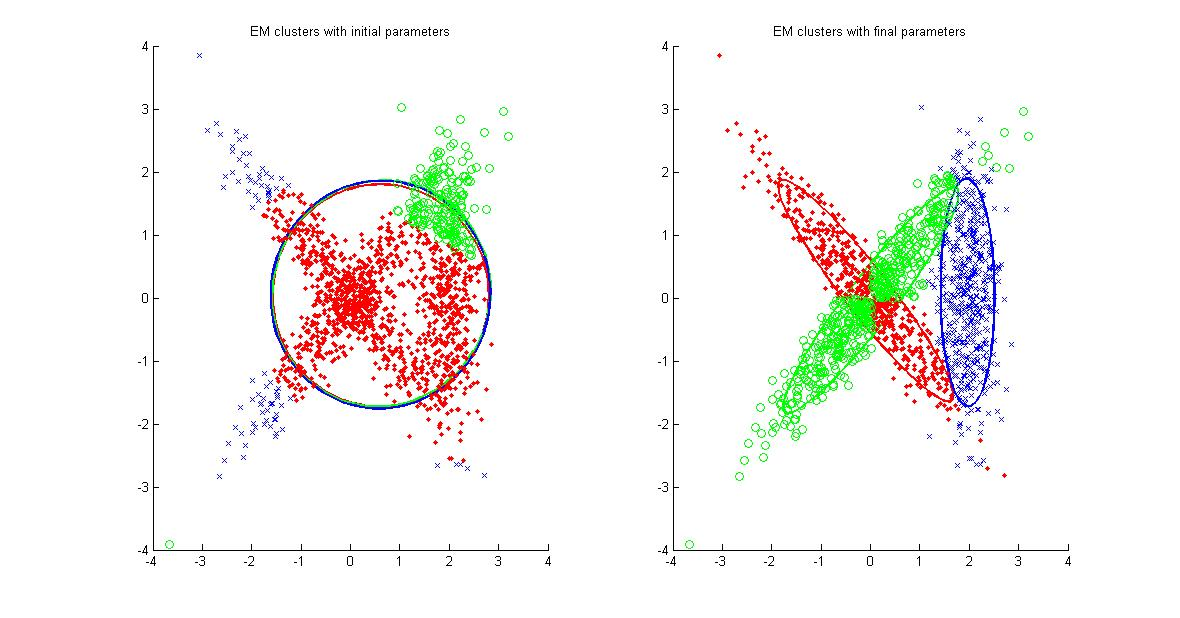
\includegraphics[height=3.25in]{dataset2_EMclusterPlots.jpg}
\caption{The EM cluster plots for dataset2, K=3, using initialization method 1}
\end{figure}

\begin{figure}[H]
\centering
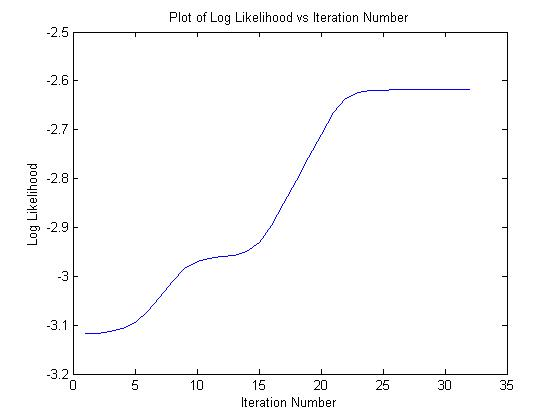
\includegraphics[height=3.25in]{dataset2_EMlogLikelihoodPlot.jpg}
\caption{The likelihood plot for dataset2, K=3, using initialization method 1}
\end{figure}

\section*{Plots for Dataset3}

\begin{figure}[H]
\centering
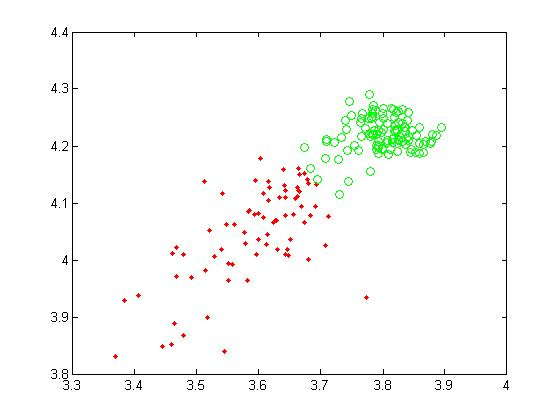
\includegraphics[height=3.25in]{dataset3_kMeansPlot.jpg}
\caption{The k-Means plot for dataset3, K=2}
\end{figure}

\begin{figure}[H]
\centering
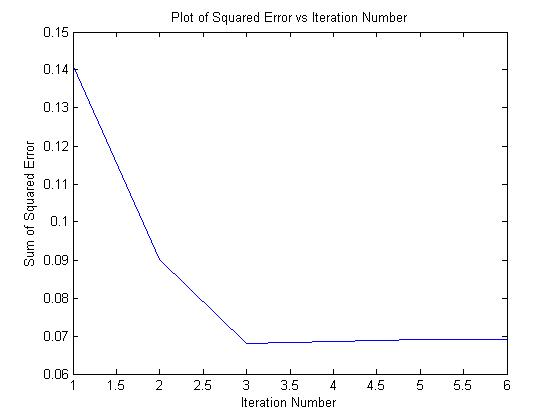
\includegraphics[height=3.25in]{dataset3_kMeans_squaredErrorPlot.jpg}
\caption{The Sum of Squared Error plot for dataset3, K=2}
\end{figure}

\begin{figure}[H]
\centering
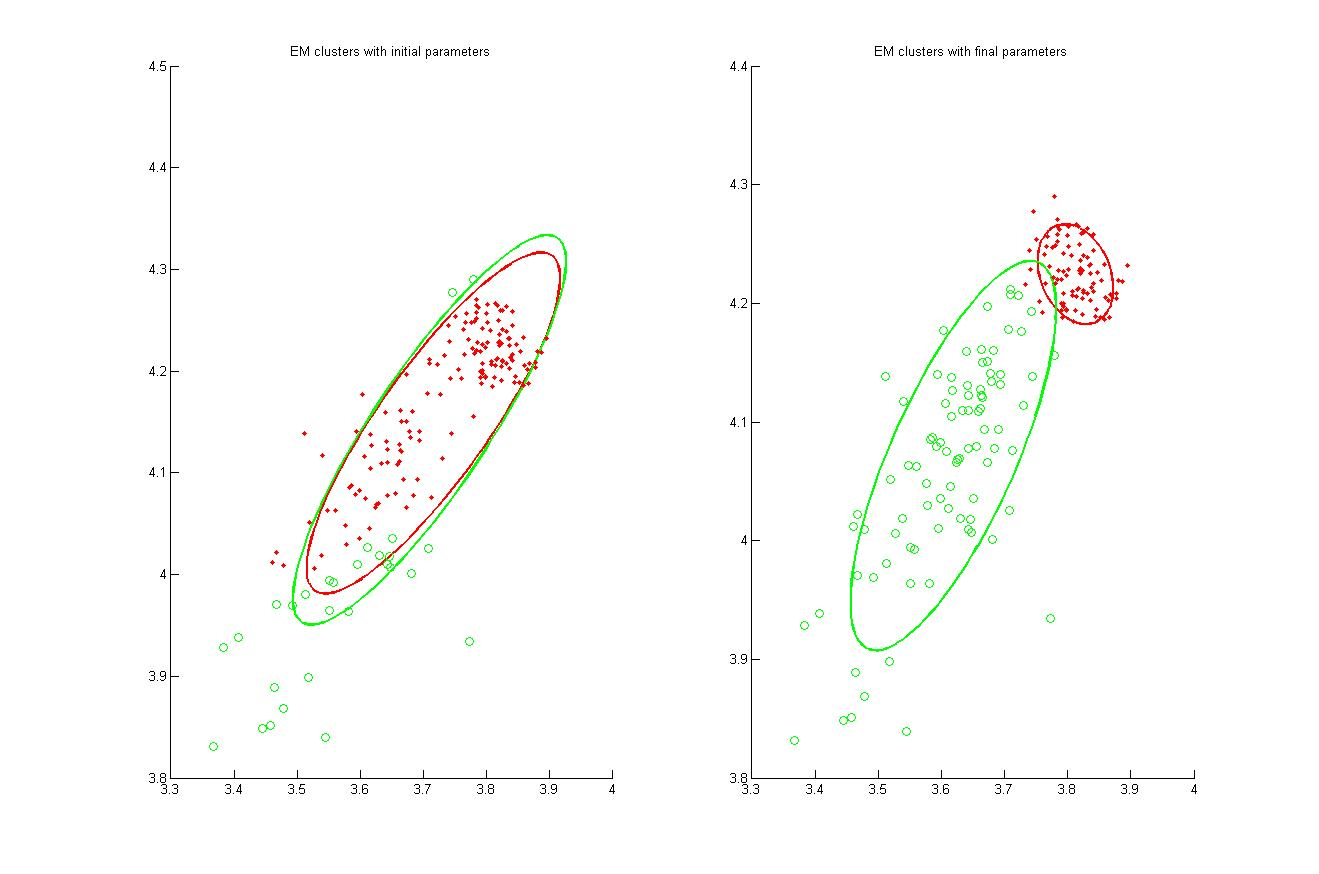
\includegraphics[height=3.25in]{dataset3_EMclusterPlots.jpg}
\caption{The EM cluster plots for dataset3, K=2, using initialization method 1}
\end{figure}

\begin{figure}[H]
\centering
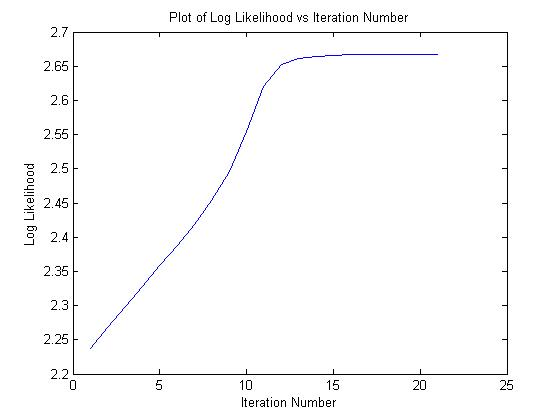
\includegraphics[height=3.25in]{dataset3_EMlogLikelihoodPlot.jpg}
\caption{The likelihood plot for dataset3, K=2, using initialization method 1}
\end{figure}

\section*{Comments on Results}

*Make new plots after comparing with Bailey*

For dataset1, there was not much of a difference between the K-means result and the EM algorithm result. This was likely due to the fact that the two Gaussians did not overlap so K-means put the points in the correct Gaussian cluster more easily. With dataset2, there was a substantial difference. The EM algorithm seemed to capture the Guassians much better than K-means. This is likely due to the fact that two of the Gaussians had an overlapping mean. Since K-means just clusters them into groups, it would not detect the differing Gaussians, whereas since EM is specifically trying to fit to Gaussians, it would detect it. For dataset3, the algorithm performed slightly better. **INSERT COMMENT ABOUT RESULT WHEN COMPARING WITH LABELSET3**

EM algorithm gives accuracy of 45.6\% for dataset 3. For k-means it was 42.3\%. 

**Mention the initialization methods used and why those could have been the best ones**

In the end, because this data was generated from Gaussian densities and the EM algorithm fits the data to Gaussians, the EM algorithm was ideally suited to find the clusters in our case. However, if our need was to put data into two groups, as with dataset3, without much knowledge of the underlying model, then k-means is the ideal solution. **INSERT COMMENT AFTER RUNNING COMPARISON WITH DATASET3**

\begin{table}[H]
  \centering
  \begin{tabular}{|c|c|c|}
    \hline
    \multicolumn{3}{|c|}{Dataset 1} \\\hline
    K & log-L & BIC \\\hline
    1 & -5459.40 & -5481.53 \\
		2 & -5344.47 & -5388.73 \\
		3 & -5343.42 & -5409.82 \\
		4 & -5341.18 & -5429.72 \\
    5 & -5337.96 & -5448.63 \\\hline
  \end{tabular}
  \begin{tabular}{|c|c|c|}
    \hline
    \multicolumn{3}{|c|}{Dataset 2} \\\hline
    K & log-L & BIC \\\hline
    1 & -4676.77 & -4698.72 \\
		2 & -4449.92 & -4493.80 \\
		3 & -3993.20 & -3993.20 \\
		4 & -3922.58 & -4010.34 \\
    5 & -3921.62 & -4031.31 \\\hline
  \end{tabular}
  \begin{tabular}{|c|c|c|}
    \hline
    \multicolumn{3}{|c|}{Dataset 3} \\\hline
    K & log-L & BIC \\\hline
    1 & 4 & 3 \\
    5 & 5 & 4 \\\hline
  \end{tabular}
\end{table}

\end{document}
